\ifieeejournal
    \documentclass[./IEEE_Journal.tex]{subfiles}
\fi 
\ifacmjournal
    \documentclass[./ACM_Journal.tex]{subfiles}
\fi 

\begin{document}
\pagenumbering{gobble} % Hide the page numbering of the subfile
\onecolumn
%================== HEADER =========================%
\vspace{2mm}
\noindent \textbf{Original Manuscript ID:} TCAS-II-YYYYY-2023  \\  
\textbf{Original Article Title:} \Paste{PaperTitle}  \\
\vspace{2mm}
\\\textbf{To:} IEEE TCAS-II Editor and Reviewers \\
\textbf{Re:} Response to reviewers \\
%====================================================%

% General intro text goes here
We are grateful to the Editor for having managed the review of our manuscript. We also want to thank the reviewers for their critical assessment of our work, and for the useful comments that help us to improve the quality of the manuscript.
In the following we address their concerns point by point. 
We are uploading (a) our point-by-point response to the comments (below) (response to reviewers), (b) an updated manuscript with \hl{yellow highlighting} indicating changes, and (c) a clean updated manuscript without highlights (Main Manuscript).

%===========================================
\reviewersection 
    Paste the general comments of the handling editor here (if given) \\
    \red{Note: the \texttt{\textbackslash reviewersection} command is used for a  response to the general (opening) comments of each reviewer.}

\replySingle{
    We thank the editor for the time spent in reviewing our work and for its general appreciation... \\
    \red{Note: the \texttt{\textbackslash replySingle} command is for writing a reply \textbf{without} adding the ``\textbf{Authors' Action}'' section.}
}

% === Concern
\begin{point}
     The first comment from Reviewer 1... \\
     \red{Copy each comment from the review letter (often sent in an email) and paste into a new \texttt{point} block.}
\end{point}

\replyFull{
    We thank the Reviewer for this comment... Indeed, \blue{the reviewer is always right!} \\
    \red{Note: the \texttt{\textbackslash replyFull} command is for writing a reply \textbf{followed by} the ``\textbf{Authors' Action}'' section. Use this if you took any actions, such as adding/modifying text, adding/modifying a figure, etc.}
}{
\begin{itemize}
    \item \blue{Use a separate \texttt{\textbackslash item} bullet for each modification in the manuscript.}
    
    \item The following text was added to \secref{sec:Sec2}, Par. 1: \\
    \red{Note: Use the \texttt{quote} environment to quote new/modified text from the manuscript. Use the \texttt{clipboard} package to \texttt{\textbackslash Copy} and \texttt{\textbackslash Paste} text from the manuscript into the reply letter. Put quotation marks around the copied text.}
    \begin{quote}
        ``\Paste{SecIPar1}''
    \end{quote}
  
     \item Based on the comment, \figref{fig_MyLabel} was updated: \\
    \red{Note: Instantiate the figure here. If the figure is appropriate for comments from several reviewers, instantiate it several times in the reply letter (though only once per reviewer). Use the \texttt{h!} position to place the figure in-line with the reply, if possible. Comment out the \texttt{\textbackslash label}, so it's not dually defined.} \\
    \red{Note 2: Use the \texttt{\textbackslash setcounter} command to make the figure numbering right. It should be one less than the number in the manuscript, so if, for example, this is Fig. 6, you should set the counter to 5 and when you instantiate the figure, it will increment by one.}
    \setcounter{figure}{5}
    
    \begin{figure}[h!] % [b]-> bottom, [t]->top, [H]->Here! ([h!] should do a better job), {figure*}->float
         \centering
         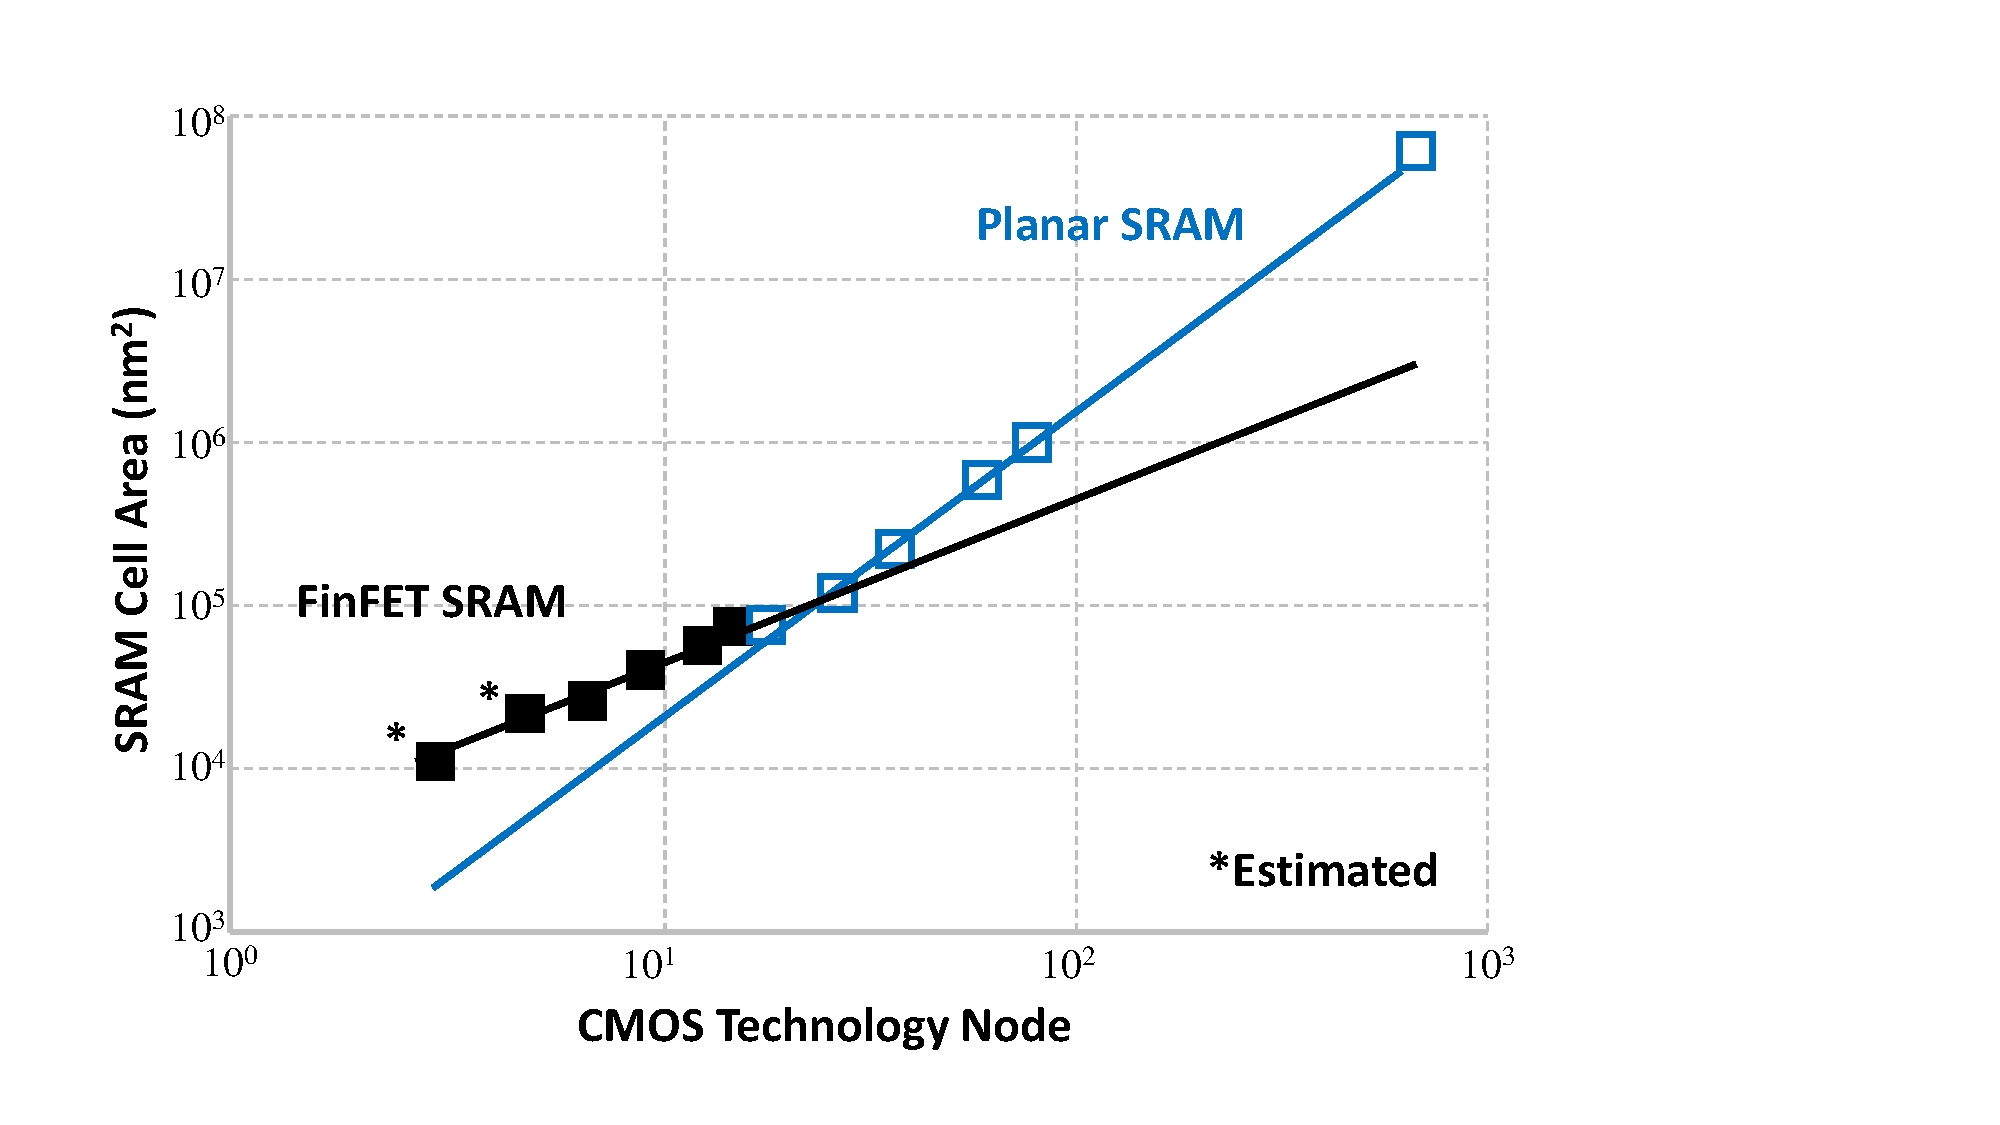
\includegraphics[width=0.5\columnwidth, trim = 0.5cm 0.2cm 0.3cm 0.3cm, clip]{example_plot}
         \caption{\red{Instantiate the new/modified figure here. You could ``Copy-Paste'' the \LaTeX code, but you will want to use a \texttt{H!} position and to comment out the label and play with the size, so better to just copy and paste the code.}}
         \label{fig_MyLabel}
    \end{figure}
\end{itemize}
}

% === Concern
\begin{point}
     Here is Reviewer 1's second concern...
\end{point}

\replySingle{
    We thank the Reviewer for this comment... \\
    \red{Note: In this case, we didn't make any modifications to the manuscript, so we used \texttt{\textbackslash replySingle} instead of \texttt{\textbackslash replyFull}}
}

%===========================================
\reviewersection 
\blue{This started the review of the second reviewer. Put Reviewer 2's general comments here (if given)} 



%\newpage
\vspace{2cm} \hrule \vspace{0.2cm} \hrule \vspace{0.5cm}

\color{magenta}

%TC:ignore
Words and characters in the response letter is detailed below. 
The text (as the text in this new page) placed within the comment flags ``TC:ignore'' and ``TC:endignore'' are not counted.
Note that this word/character count does not include the text copied from the main manuscript.

\begin{itemize}
    \item Response letter word count: \quickwordcount{A2R}
    \item Response letter character count: \quickcharcount{A2R}
\end{itemize}

\par{Detail count follows:}
% \detailtexcount{Reply_To_Reviewers}
% \detailtexcount{IEEE_Journal}
%TC:endignore

\color{black}







\twocolumn


\section{Response Letter Overview}\label{sec:overview}
The response letter is named ``Answer to Reviewers'' or ``A2R''.
It uses two input files, which must be loaded in the main manuscript in order to set the correct formatting of the response letter that is called as ``\textbackslash subfile\{A2R\}'' before the ``\textbackslash end\{document\}''.
A brief description of the two input files follows:
\begin{itemize}
    \item \textbf{A2R\_environment.tex}: it includes all the extra packages, definition of counters for reviewers and their point-by-point concerns, environment (letter format), and commands, related to the A2R response letter.
    \item \textbf{A2R\_inputs.tex}: all the details of the submitted paper have to be written in this file. 
\end{itemize}

\subsection{Commands}
\begin{enumerate}
    \item \textbackslash reviewersection: It generates a Reviewer block/section
    \item \textbackslash replySingle\{\#1\}: This command receives one input (\#1). This input is the reply to the reviewer. By default the answer is written in blue. 
    \item \textbackslash replyFull\{\#1\}\{\#2\}: This command receives two inputs (\#1 and \#2). The former input is the reply to the reviewer, while the latter is the changes that we did to the manuscript. By default the answers are written in blue.
\end{enumerate}
An example of this commands are presented in the A2R.tex file.


\subsection{Use of highlighting}
Use the ``\textbackslash hl\{\}'' to highlight some text. 
It may be problematic if you highlight a text that presents some commands within it. To address this, it is suggested to close the command between ``\{\}'' or ``\textbackslash mbox\{\}'' 

\subsection{Use of Copy-Paste commands}
Within the A2R\_environment.tex file is loaded a package that allows to ``copy'' and ``paste'' pieces of text from one document to another.
\textbf{It is suggested to use ``copy'' command within the main manuscript and ``paste'' such a text in the changes block of the A2R letter.}
In this way, it will save time and avoid possible human errors.
A brief description of the Copy-Paste commands follows:
\begin{itemize}
    \item \textbackslash Copy\{\#1\}\{\#2\}: It receives two inputs (\#1 and \#2). The former input is the name of the copied text. The latter is the text we want to copy.
    \item \textbackslash Paste\{\#1\}: It receives one input (\#1). It is the name of the text we want to paste. The name has to match the name used with the ``Copy'' command.
\end{itemize}

\section{Section 2: Example of Copy-Paste}\label{sec:Sec2}
In the paragraph bellow is an example of the ``copy'' command. The ``paste'' command is used in A2R.tex file.

\subsection{Automatic generation of A2R file}
To ease some work, \href{https://github.com/EstebanJGC/Latex_Templates_Macros.git}{\red{here}}  you can find a python script (named \textit{generateA2R.py}) that partially generates the A2R file for $n$ reviewers, each one with a given number of concerns. 

\lipsum[50].


 
\section{Conclusion}\label{sec:conclusion} 



\end{document}
